%!TEX root = main.tex

\section{Results and discussion}

Molecular weight, viscosity, density, and thermal conductivity of the individual gases investigated in this paper are shown in Figure \ref{fig:gas-properties}. The gas properties were calculated at a pressure of 101,325 Pa and a temperature of 773.15 K (500$^\circ$C). The lightest gas in terms of molecular weight and density is hydrogen while the heaviest gas is carbon dioxide. Viscosity for all the gases except hydrogen ranged from 300--350 \textmugreek P. Thermal conductivity for all the gases is near 0.05 W/(m\,K) except for hydrogen which is approximately 0.35 W/(m\,K).

\begin{figure}[H]
    \centering
    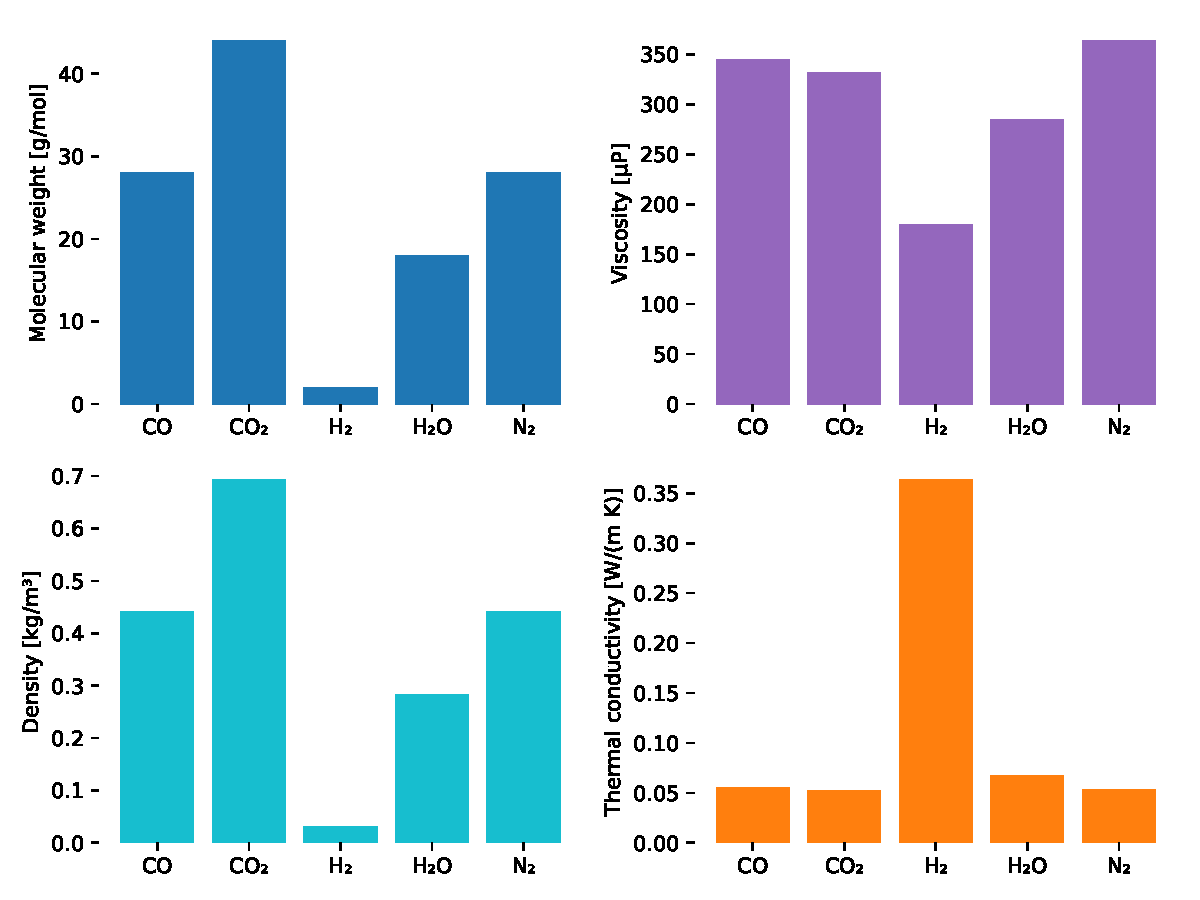
\includegraphics[width=\textwidth]{gas-properties.pdf}
    \caption{Comparison of molecular weight, viscosity, density, and thermal conductivity for individual gases at 101,325 Pa and 773.15 K.}
    \label{fig:gas-properties}
\end{figure}

Properties for molecular weight, viscosity, and density for the gas mixtures investigated in this paper are shown in Figure \ref{fig:mix-properties}. Similar to the individual gas properties, the mixture properties were calculated at 101,325 Pa and 773.15 K (500$^\circ$C). The fraction of each gas in the mixture is given by the values shown at the top of each column in the figure. For example, the hydrogen and nitrogen mixture is comprised of 80\% hydrogen and 20\% nitrogen which is labeled as $0.8 + 0.2$. As expected, the carbon dioxide mixture is the heaviest in terms of molecular weight and density.

\begin{figure}[H]
    \centering
    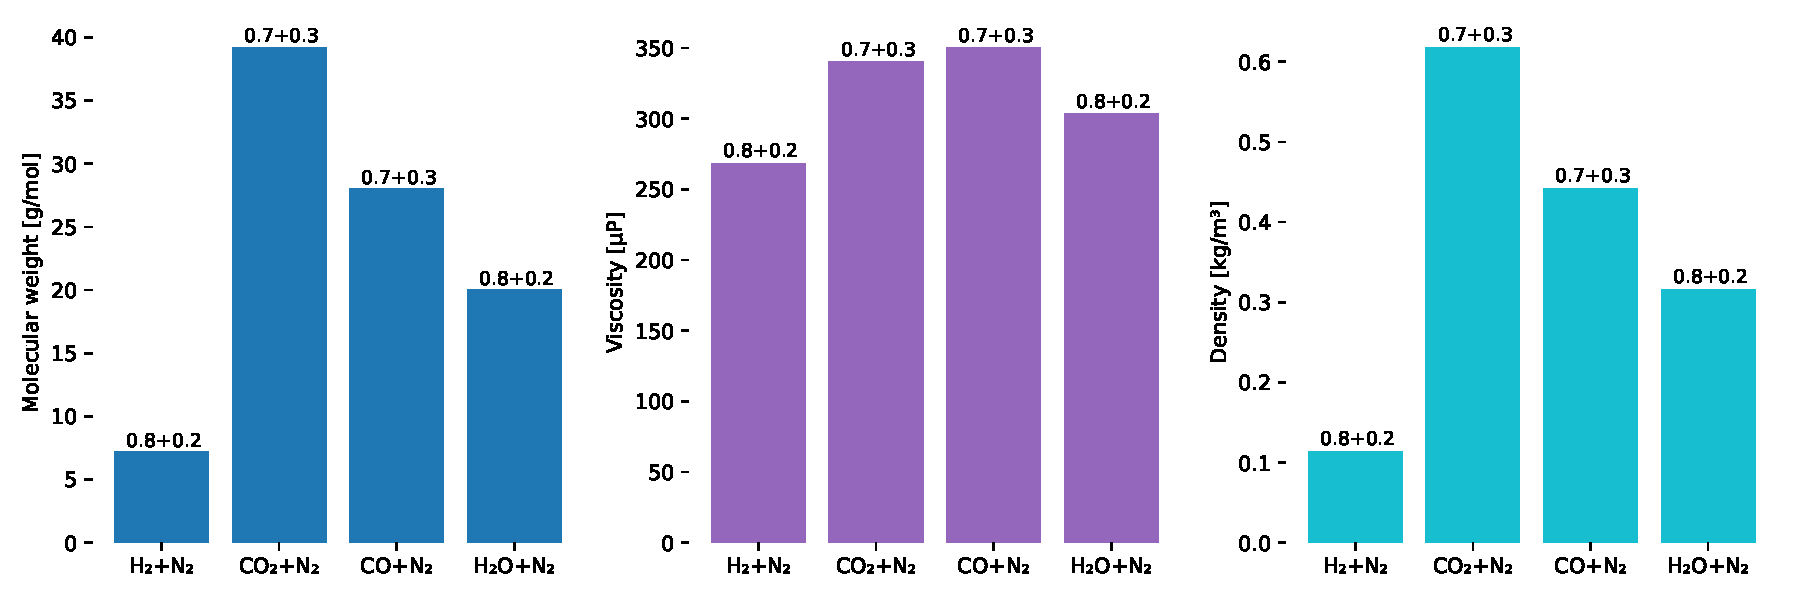
\includegraphics[width=\textwidth]{mix-properties.pdf}
    \caption{Comparison of gas mixture properties for molecular weight, viscosity, and density at 101,325 Pa and 773.15 K. Fraction of each gas component is shown at the top of each column.}
    \label{fig:mix-properties}
\end{figure}
